\documentclass{beamer}
\usepackage{pgfpages} % Used for show notes
% use this instead for 16:9 aspect ratio:
%\documentclass[aspectratio=169]{beamer}

\providecommand{\main}{.} % relative path to master.tex

\graphicspath{{../../reports/Thesis/Pictures/}} % Specifies the directory where pictures are stored

\makeatletter
\providecommand*{\input@path}{{..}}
\g@addto@macro\input@path{{..}}% append % if you cant override it
\makeatother

%General Remarks
%- Tell a story i.e. build your presentation around a small set of messages you want to communicate. Think about what you want to tell.
%- Tailor your presentation to your audience. How much do they know - what needs to be explained and what not? What are they interested in?
%- Make sure that the main messages of your slides can also be understood by a deaf person following your presentation
%- Don’t put too much text on your slides. Stick with short messages

%Animations
%- It’s a scientific presentation so only use subtle animations (no motion, no blinking)

%Structure
%- Make sure that you guide the eye of the viewer to the things you want to communicate
%- Distribute your content among slides rather than overfilling one
%- Make the content appear step by step to guide the viewer through it (Animations - Fade In)
%- Do not use background images or strong background colors
%- If you have a date on your slides, make sure it is correct
%- Don’t put logos in the footer of your slides

%Fonts
%- The fonts have to be big enough be be readable even from far away - min. 20 pt (also for figure captions)
%- Comic sans is the right font for birthday cards but not for presentations

%Figures
%- Make sure the axes are labeled correctly and they have to be readable

%Hint: Display your talk on your laptop. Now walk to the other side of the room. Can you still read everything?

%Slide Titles
%- The title should be short and descriptive: What is the content of the slide?
%- Substantives have to be upper case in a title

%Headers / Footers
%- Put numbers on your slides so that people with questions car refer to them
%- Keep your headers and footers as minimal as possible otherwise they are distractors. At ISSCC for example, all logos, footers etc are BANNED.

%Movies / Live Demos
%- If you have movies of your work - show them!
%- If you have demos of your work, you first have to make sure that they run under the given conditions. Do not rely on them to work. Avoid showing demos that do not run robustly. If your demo is not reliably working, take a movie.

%% LaTeX Font encoding -- DO NOT CHANGE
\usepackage[OT1]{fontenc}

%% Babel provides support for languages.  'english' uses British
%% English hyphenation and text snippets like "Figure" and
%% "Theorem". Use the option 'ngerman' if your document is in German.
%% Use 'american' for American English.  Note that if you change this,
%% the next LaTeX run may show spurious errors.  Simply run it again.
%% If they persist, remove the .aux file and try again.
\usepackage[english]{babel}

%% Input encoding 'utf8'. In some cases you might need 'utf8x' for
%% extra symbols. Not all editors, especially on Windrows, are UTF-8
%% capable, so you may want to use 'latin1' instead.
\usepackage[utf8]{inputenc}

%% This changes default fonts for both text and math mode to use Herman Zapfs
%% excellent Palatino font.  Do not change this.
\usepackage[sc]{mathpazo}


%% We unfortunately need this for the Rules chapter.  Remove it
%% afterwards; or at least NEVER use its underlining features.
\usepackage{soul}
\usepackage{bm}
\usepackage{datetime}
%% To use alternating colors in the glossary
\usepackage[table]{xcolor}
%% We use subfiles to separate the file into subfiles which are compilable on their own by copying the preamble from this file.
\usepackage{subfiles}

%common
\usepackage{comment}
\usepackage{ifthen}
\usepackage{todonotes}
% to disable the todo notes in the final version in case we still have to do notes
\presetkeys{todonotes}{disable}{}

\usepackage{titlesec}

%lists
\usepackage{listings}
\usepackage{enumerate}


%plain text
\usepackage{verbatim} %% many common packages

%% See the TeXed file for more explanations

%% [OPT] Multi-rowed cells in tabulars
\usepackage{multirow}

%% [REC] Intelligent cross reference package. This allows for nice
%% combined references that include the reference and a hint to where
%% to look for it.
\usepackage{varioref}

%% [OPT] Easily changeable quotes with \enquote{Text}
%\usepackage[german=swiss]{csquotes}

%% [REC] Format dates and time depending on locale
\usepackage{datetime}

%% [OPT] Provides a \cancel{} command to stroke through mathematics.
\usepackage{cancel}

%% [NEED] This allows for additional typesetting tools in mathmode.
%% See its excellent documentation.
\usepackage{mathtools}

%% [ADV] Conditional commands
%\usepackage{ifthen}

%% [OPT] Manual large braces or other delimiters.
%\usepackage{bigdelim, bigstrut}

%% [REC] Alternate vector arrows. Use the command \vv{} to get scaled
%% vector arrows. (package texlive-fonts-extra)
\usepackage[h]{esvect}

%% [NEED] Some extensions to tabulars and array environments.
\usepackage{array}

%% [OPT] Postscript support via pstricks graphics package. Very
%% diverse applications.
%\usepackage{pstricks,pst-all}

%% [?] This seems to allow us to define some additional counters.
%\usepackage{etex}

%% [ADV] XY-Pic to typeset some matrix-style graphics
%\usepackage[all]{xy}

%% [OPT] This is needed to generate an index at the end of the
%% document.
%\usepackage{makeidx}

%% [OPT] Fancy package for source code listings.  The template text
%% needs it for some LaTeX snippets; remove/adapt the \lstset when you
%% remove the template content.
\usepackage{listings}
\lstset{language=TeX,basicstyle={\normalfont\ttfamily}}

%% [REC] Fancy character protrusion.  Must be loaded after all fonts.
\usepackage[activate]{pdfcprot}

%% [REC] Nicer tables.  Read the excellent documentation.
\usepackage{booktabs}

%% International System measurement units (package texlive-science)
\usepackage{siunitx}

%% Subfigures
%\let\subcaption\undefined
%\let\subfloat\undefined
%\usepackage{subcaption}

%section customisation
\usepackage{titlesec}

%% Advanced figures
\usepackage{tikz}

%% Electronics circuits
%\usepackage[arrowmos]{circuitikz}

%%Image position
\usepackage{float}

%%Long tables
\usepackage{longtable}
\usepackage{tabu}

%% LaTeX' own graphics handling
\usepackage{graphicx}

%% The AMS-LaTeX extensions for mathematical typesetting.  Do not
%% remove.
\usepackage{amsmath,amssymb,amsfonts,mathrsfs,amscd,xspace}

%% NTheorem is a reimplementation of the AMS Theorem package. This
%% will allow us to typeset theorems like examples, proofs and
%% similar.  Do not remove.
%% NOTE: Must be loaded AFTER amsmath, or the \qed placement will
%% break
\usepackage[amsmath,thmmarks]{ntheorem}

%different enumerations
\usepackage{enumitem}

%% Make document internal hyperlinks wherever possible. (TOC, references)
%% This MUST be loaded after varioref, which is loaded in 'extrapackages'
%% above.  We just load it last to be safe.
\usepackage[linkcolor=black,colorlinks=true,urlcolor=black,citecolor=black,filecolor=black]{hyperref}


\input{glyphtounicode}
  \pdfgentounicode=1
\usepackage{cmap}

\usepackage{accsupp}
\usepackage{calc}
\usepackage{layouts}
\usepackage{layout}

 
\mathtoolsset{showonlyrefs}  

% Lorem ipsum
%\usepackage[]{blindtext}
\usepackage{lipsum}% dummy text
% include pdfs into the latex document
\usepackage{pdfpages}
%for landscape cheatsheet
\usepackage{pdflscape}


% Units
\usepackage{units}

% tables
\usepackage{array}
\usepackage{rotating}
\usepackage{longtable}

%layout
\usepackage{multicol}
\setlength{\columnseprule}{0.4pt}
\usepackage{chngpage}
 %% Some more packages that you may want to use.  Have a look at the
%% file, and consult the package docs for each.

%% We use subfiles to separate the file into subfiles which are compilable on their own by copying the preamble from this file.
\usepackage{subfiles}
\usepackage{etex}
\reserveinserts{28}
\usetheme{ETHbeamer}

\colorlet{ETHcolor1}{ETHc}
\colorlet{ETHcolor2}{ETHc}

%\setbeameroption{show notes}
\setbeameroption{show notes on second screen=right}

%Title Slide
%- Put the logos of the institutions you are affiliated with on the title slide. Leave them away in the following slides.
%- Your name and the occasion of the presentation should be mentioned on the title slide
%- Check that the date is right if mentioned

\author{Benjamin Ellenberger}

\title{Emergent Gait Periodicity in Evolved Creatures on Unknown Terrain}

\date{2015-05-18}

% uncomment if you do not want to use a department logo
%\deplogofalse

\begin{document}

\titleframe

%########################
%Introduction
%- After a short Welcome, the audience has to be introduced to the question which you are going to answer in the talk or the story you are going to tell. Why is what you you present of relevance?
%- For longer talks, it is better to start with an overview slide that explains the structure of the talk
\subfile{sections/01.Introduction/Introduction.tex}

%########################
%Methods
%- After the Introduction you explain what you did
%########################
%Results
%- As soon as the audience knows what you did, you show them what you got
%- Quantify in a understandable way - explain your measures
\subfile{sections/02.3DVCE-Simulation/3DVCE-Simulation.tex}
\subfile{sections/03.Chaos/Chaos.tex}
\subfile{sections/04.Mathematica/Mathematica.tex}
\subfile{sections/05.ModelLeg/ModelLeg.tex}
\subfile{sections/06.Simulations/Simulations.tex}

%########################
%Discussion
%- Discuss what you got
\subfile{sections/07.Discussion/Discussion.tex}

%########################
%Conclusion
%- Contextualize and summon your findings
%- Refer back to your introduction
%- Sell your findings to the audience - everyone should walk out of the room with the good feeling that they learned something
\subfile{sections/08.Conclusion/Conclusion.tex}

%########################
%Outlook
%- Present the next steps
\subfile{sections/09.Outlook/Outlook.tex}

%########################
%Acknowledgements
%- Thank your colleagues 
%- Thank the funding institutions for the money
%- Thank the audience for their attention (not necessary for conferences)
%- If you put pictures of the main contributors of the presented work on the acknowledgement slide, it’s easier for the audience to associate them to the work presented.
%- It’s also fair and sometimes even mandatory to mention your funding institutions (incl. logo?) on one of the last slides
\subfile{sections/10.Acknowledgements/Acknowledgements.tex}

%########################
%Backup Slides
%- Keep some supplementary material on backup slides to reply on questions on content which you were not capable of presenting (due to the restricted time)
\subfile{sections/11.Backup-Slides/Backup-Slides.tex}

\begin{comment}
\begin{frame}

  \frametitle{Contents}
  \tableofcontents[currentsection]
\end{frame}
\note{Hello world}


\section{Something}

\frame{

  \frametitle{Evolving Virtual Creatures}
  
  \begin{columns}
   \column{0.3\textwidth}
 \begin{itemize}
	     \item a
    	\item b
    	\item c
     \end{itemize}
     
     \column{0.6\textwidth}
      %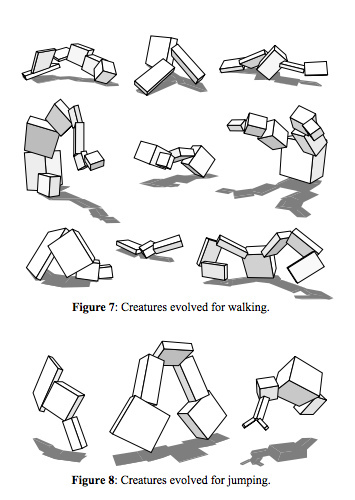
\includegraphics[width=2in, clip] {figs/creatures.jpg} 
  \end{columns}
  }
\note{}

\begin{frame}
\textbf{New colors and their names\\}
Here we show the different colors you can use. From left to right, this are the colors ETH1, ETH2, \ldots , ETH9.

\newcommand{\quadrat}{(0,0mm)--(0mm,5mm)--(5mm,5mm)--(5mm,0mm)--(0mm,0mm);}
\begin{center}
	\hspace{-8mm}
	\begin{tikzpicture}[overlay]
		{\draw[ETHa,fill=ETHa] \quadrat}\label{ETH1}
	\end{tikzpicture}
	\hspace{10mm}
	\begin{tikzpicture}[overlay]
		{\draw[ETHb,fill=ETHb]\quadrat}\label{ETH2}
	\end{tikzpicture}
	\hspace{10mm}
	\begin{tikzpicture}[overlay]
		{\draw[ETHc,fill=ETHc]\quadrat}\label{ETH3}
	\end{tikzpicture}
	\hspace{10mm}
	\begin{tikzpicture}[overlay]
		{\draw[ETHd,fill=ETHd] \quadrat}\label{ETH4}
	\end{tikzpicture}
	\hspace{10mm}
	\begin{tikzpicture}[overlay]
		{\draw[ETHe,fill=ETHe] \quadrat}\label{ETH5}
	\end{tikzpicture}
	\hspace{10mm}
	\begin{tikzpicture}[overlay]
		{\draw[ETHf,fill=ETHf] \quadrat}\label{ETH6}
	\end{tikzpicture}
	\hspace{10mm}
	\begin{tikzpicture}[overlay]
		{\draw[ETHg,fill=ETHg] \quadrat}\label{ETH7}
	\end{tikzpicture}
	\hspace{10mm}
	\begin{tikzpicture}[overlay]
		{\draw[ETHh,fill=ETHh] \quadrat}\label{ETH8}
	\end{tikzpicture}
	\hspace{10mm}
	\begin{tikzpicture}[overlay]
		{\draw[ETHi,fill=ETHi] \quadrat}\label{ETH9}
	\end{tikzpicture}
\end{center}

Please use no more then two of them in your presentation. The first two (counted from the left hand side) are reserved for the administration chapter of the ETHZ (first one for external presentation, second for internal), all others you can freely choose.

\end{frame}

\begin{frame}
\textbf{Some mathematical specialities}

\ETHbox{0.8\textwidth}{% define the ETHbox
  \begin{theorem}[Murphy (1949)]\label{murphy}
    Anything that can go wrong, will go wrong.
  \end{theorem}
}

\begin{proof}
  A special case of Theorem \ref{murphy} is proven in %\citet{matthews1995}.
\end{proof}
\end{frame}

\begin{titlestyleframe}
\frametitle{Title Page}

\color{white} The title page is created using the \texttt{\textbackslash titleframe} command.

The title page background can also be used on other frames (or for a customised title frame) using the \texttt{titlestyleframe} environment.
\end{titlestyleframe}

\begin{frame}
\frametitle{Normal Frame}
The normal frame looks like this. It is created using the \texttt{frame} environment.
\end{frame}
\begin{inverseframe}
  \frametitle{Inverse Slides}
  %\color{white}
The inverted frame looks like this. It is created using the \texttt{inverseframe} environment.

 
\end{inverseframe}

\begin{minimalframe}
  \frametitle{Minimal Frame}
The minimal frame looks like this. It is created using the \texttt{minimalframe} environment.
  
\end{minimalframe}

\end{comment}

\end{document}
